%!TEX root = ../USthesis_Masters.tex
\chapter{Detail Design}
\label{chp:Detail Design}


%%%%%%%%%%%%%%%%%%%%%%%%%%%%%%%%%%%%%%%%%%%%%%%%%%%%%%%%%%%%%%%%%%%%%%%
\section{Back-end}

To implement the payment framework, we need a back-end server and a back-end web framework. 

\subsection{Back-end Server}

We chose an Amazon Elastic Cloud Computing (EC2) instance for the back-end server. EC2 gives us access to a virtual machine (VM) where we can run our own software, including a publicly accessible website. The micro instance is deployed in Singapore in the Asia Pacific region. The reason for this is to have the server as close as possible to the WeChat servers in China, since our servers must connect to WeChat's servers.

\subsection{Back-end Web Framework}

We decided to use XAMPP (Apache, MySQL, PHP and Perl) for the back-end development environment. XAMPP is a full stack development environment. It includes an HTTP server (Apache), a database server (MySQL) and a scripting language (PHP). XAMPP is free and easy to deploy, and is also used because the author is familiar with it.

\section{Social Media Platform}

We chose WeChat for our social media platform. WeChat works on most smartphones, already has a userbase and it has a third-party API with a development sandbox feature. 

On WeChat, a third-party application is known as an ``Official Account''. We registered for a sandbox Official Account that only allows 20 users and is not searchable on WeChat.

WeChat acts as an intermediary between the user and our server as seen in figure \ref{fig:wechat_interaction}. 

\begin{figure}
  \centering
    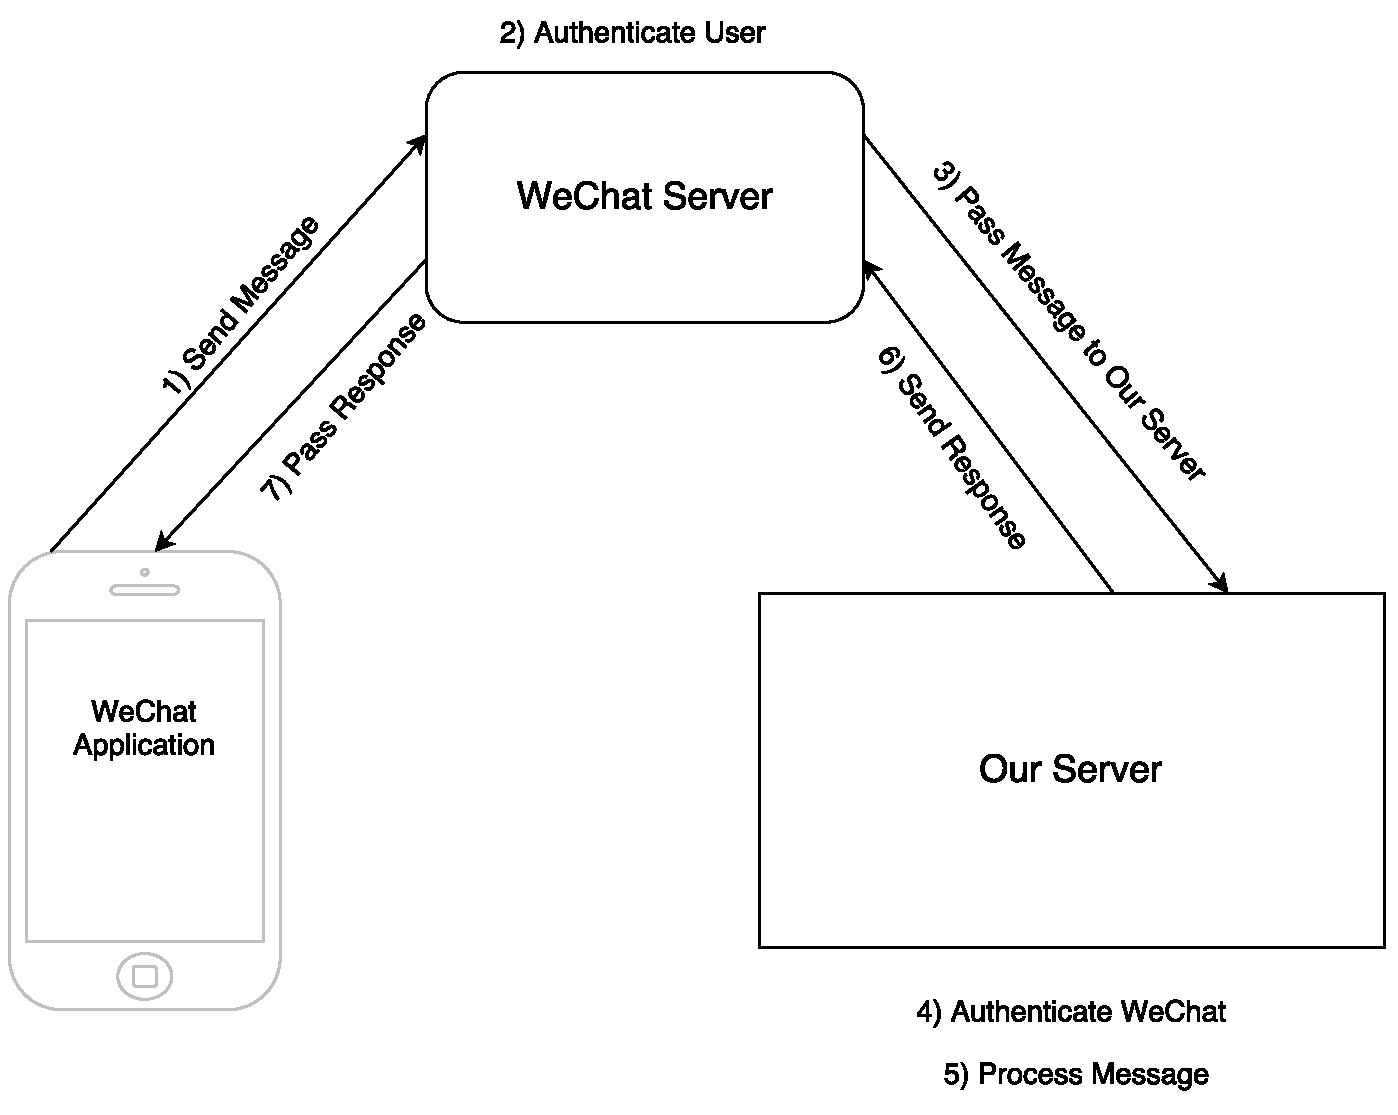
\includegraphics[width=0.7\textwidth]{figs/Wechat_interaction.pdf}
   \caption{Interaction with WeChat} 
   \label{fig:wechat_interaction}
\end{figure}

WeChat uses a shared token hashing scheme to authenticate itself on our service. We provide 